\section{What the re-solve move converges to}
\label{sec:legacy}

\subsection{The move}

The move we analyse is natural, and a version of it was the spectral-index step of the per-pixel
path in the development version of Commander4 that we started from (option
\texttt{resolve\_chisq} in our branch). Given the current $(\beta, a)$:
\begin{enumerate}
  \item propose $\beta'$ from a symmetric random walk;
  \item draw new amplitudes from their conditional at the proposed index,
        $a' \sim \mathcal{N}\!\big(\hat a(\beta'), \A(\beta')^{-1}\big)$;
  \item accept $(\beta', a')$ with probability $\min\{1, \exp[-(\chi^2(\beta',a') - \chi^2(\beta,a))/2]\}$.
\end{enumerate}
The Gibbs sweep then continues with the amplitude group, which redraws
$a \sim \mathcal{N}(\hat a(\beta), \A(\beta)^{-1})$, and possibly repeats the index move $n$ times before
that. The intent is to move the index and the amplitudes together and so avoid the slow mixing of the
conditional index step. Write $X = (a-\hat a)\T \A (a-\hat a)$, so that
$\chi^2 = \chimin(\beta) + X$ by Eq.~(\ref{eq:chisplit}). For an amplitude draw from the conditional,
$X \sim \chi^2_k$ whatever $\beta$ is.

\subsection{Alone, the move is exact for the profile posterior}

Because $\E[\exp(-X/2)] = 2^{-k/2}$ does not depend on $\beta$, the quantity
$\exp[-\chi^2(\beta, a)/2]$ at a fresh conditional draw is an unbiased estimator of
$\mathcal{L}_{\rm prof}(\beta)$ up to a constant. Steps 1 to 3, with the accepted amplitudes kept as
part of the state, are therefore a pseudo-marginal Metropolis-Hastings kernel
\citep{beaumont2003,andrieu2009}. Its extended target is
\begin{equation}
  \pi(\beta, a) \propto p(\beta)\, \exp\!\left[-\tfrac12\chimin(\beta)\right]\,
  \det\A(\beta)^{1/2} \exp\!\left[-(a-\hat a)\T \A\, (a-\hat a)\right],
  \label{eq:extended}
\end{equation}
whose index marginal is the profile posterior and whose amplitude conditional is
$\mathcal{N}(\hat a, (2\A)^{-1})$: the amplitudes carry half their posterior covariance. So the move
does have a target, the target is the profile posterior, and the determinant never enters. This is why
chains run with this move have means close to the profile posterior. Under
Eq.~(\ref{eq:extended}), $X \sim \mathrm{Gamma}(k/2, 1)$ with mean $k/2$.

\subsection{The amplitude step of the Gibbs sweep breaks it}

The amplitude group redraws $a$ with the full conditional covariance $\A^{-1}$, which resets $X$ to a
$\chi^2_k$ variate with mean $k$. That is the conditional of the flat-prior joint posterior and not of
Eq.~(\ref{eq:extended}). The two kernels share no invariant distribution. With one index move per
amplitude draw, both the current and the proposed estimate are fresh at every index move, and the
composite is Monte Carlo within Metropolis in the terminology of \citet{andrieu2009}, following
\citet{oneill2000} and \citet{beaumont2003}. \citet{andrieu2009} note that the target is typically
not the invariant density of such a chain and that the existence of an invariant distribution is not
obvious in general. Here it can be written down.

\subsection{The stationary law: a tempered profile posterior}

With one move per amplitude draw the index chain is Markov on its own, with acceptance probability
\begin{equation}
  \alpha(D) = \E\big[\min\{1, e^{-(D+Z)/2}\}\big], \qquad
  D = \chimin(\beta') - \chimin(\beta) - 2\ln\frac{p(\beta')}{p(\beta)}, \qquad Z = X' - X ,
\end{equation}
where $X$ and $X'$ are independent $\chi^2_k$ variates, so $Z$ is symmetric with variance $4k$. In the
limit of small proposal steps the chain is a diffusion with drift proportional to $\alpha'(0)$ and
diffusion coefficient proportional to $\alpha(0)$, and its stationary density is
\begin{equation}
  \pi(\beta) \propto \left\{ p(\beta) \exp\!\left[-\tfrac12\chimin(\beta)\right] \right\}^{1/T},
  \qquad T = \frac12 + \frac{1}{4 c_k}, \qquad
  c_k = \E\big[e^{-Z/2};\, Z > 0\big] = 2^{-(k+1)} \binom{k}{k/2} .
  \label{eq:Tk}
\end{equation}
The formula is exact for every $k$ and every shape of $\chimin$ in the small-step limit; $T(0) = 1$
recovers Metropolis. For large $k$,
\begin{equation}
  T = \sqrt{\frac{\pi k}{8}} + \frac12 + O(k^{-1/2}) ,
  \label{eq:Tlarge}
\end{equation}
so the index posterior is the profile posterior with its width multiplied by
$\sqrt{T} \simeq 0.79\, k^{1/4}$. The stationary acceptance rate is $\tfrac12 + c_k$, close to one half
and independent of the step size, which is why such a chain looks healthy.

Equation~(\ref{eq:Tk}) does not need $\chi^2_k$ noise. For any symmetric acceptance noise $Z$ with
density $f_Z$, $T \simeq \tfrac12 + 1/(8 f_Z(0))$, and for Gaussian noise
\begin{equation}
  T \simeq \frac12 + \sqrt{\frac{\pi}{8}}\; \sigma_E , \qquad \sigma_E = \tfrac12\,\mathrm{sd}(Z) ,
  \label{eq:Tsigma}
\end{equation}
with $\sigma_E$ the standard deviation of the noise in the estimated energy difference, equal to
$1/\sqrt2$ times the standard deviation of the $\chi^2$ at a fresh amplitude draw. The leading term
is the effective temperature that \citet{ball2003} derived for the sign rule (accept if and only if
the noisy energy difference is negative; their Eq.~7), and that \citet{bardenet2017} recover without
assuming Gaussian noise (their Sect.~6.3). The Metropolis rule on the same noisy difference adds the
$\tfrac12$. Equation~(\ref{eq:Tsigma}) is the form to use when the stored amplitudes are not the drawn
ones, as below.

\paragraph{Several index moves per amplitude draw.} After the first accepted move the retained $X$ is
no longer fresh: it is biased low, and the next proposal has to beat it. In the large-$k$ limit the
accepted moves are the lower records of the sequence of fresh $X$ values, the $j$-th proposal after a
redraw is accepted with probability $1/(j+1)$, and the stationary law remains a power of the profile
posterior with temperature $T_n = R_n T_1$,
\begin{equation}
  R_n = \frac{H_{n+1} - 1}{\sqrt{\pi}\; N_\varphi(n)} , \qquad
  N_\varphi(n) = \sum_{j=1}^{n} j \int \varphi(t)^2\, [1 - \Phi(t)]^{\,j-1}\, \dd t ,
  \label{eq:Rn}
\end{equation}
where $H_n$ is the harmonic number, $\varphi$ and $\Phi$ are the standard normal density and distribution
function, and $N_\varphi(n)$ is the sum over proposals of the expected density at the running minimum.
$R_2 = 5/6$ exactly, and numerically
$R_n = 0.833$, $0.647$, $0.543$, $0.467$ and $0.357$ for $n = 2$, 5, 10, 20 and 100: more index
moves narrow the law only as $(\ln n)^{-1/4}$ in width, and the $k^{1/4}$ scaling is untouched.

\paragraph{The repair that is exact and useless.} Redrawing the amplitudes with half their covariance,
$a \sim \mathcal{N}(\hat a, (2\A)^{-1})$, is the conditional of Eq.~(\ref{eq:extended}) and makes the
composite exact for the profile posterior. Its acceptance rate at fixed index is
$2 I_{1/3}(k/2, k/2)$, with $I$ the regularized incomplete beta function, which decays as
$e^{-0.059 k}$: $6\times10^{-4}$ at $k = 100$. The useful repairs evaluate
Eq.~(\ref{eq:Lprof}) or Eq.~(\ref{eq:Lflat}) directly in the acceptance, which costs one extra
log-determinant per proposal at most (Sect.~\ref{sec:impl}).

\subsection{Tests}

\begin{table}
\centering
\caption{Variance of the stationary index distribution of the composite chain in units of the profile
posterior variance, one index move per amplitude draw, for $\chimin = \beta^2$ and exact $\chi^2_k$
refreshes. Columns: Eq.~(\ref{eq:Tk}); its leading term; the stationary vector of the exact kernel on
a grid of 1201 points, with the acceptance function computed by convolution of the $\chi^2_k$ density;
and a simulation of $10^4$ chains with a proposal step of $0.1\sqrt{T}$ (\exref{E035}, independent
review). The grid and the simulation sit 0.1 to 0.2 percent below the law because of the finite step.
Controls: with no refresh, or with a refresh from $\mathrm{Gamma}(k/2,1)$, the variance is $1.000 \pm
0.001$ at $k = 4$, 8 and 16.}
\label{tab:toy}
\begin{tabular}{rrrrrr}
\toprule
$k$ & $T$, Eq.~(\ref{eq:Tk}) & $\sqrt{\pi k/8}$ & exact kernel & simulation & acceptance \\
\midrule
10 & 2.532 & 1.982 & 2.524 & $2.525 \pm 0.008$ & 0.621 \\
100 & 6.782 & 6.267 & 6.769 & $6.751 \pm 0.024$ & 0.538 \\
1\,000 & 20.32 & 19.82 & 20.29 & $20.26 \pm 0.07$ & 0.511 \\
10\,000 & 63.17 & 62.67 & 63.07 & $63.30 \pm 0.23$ & 0.503 \\
100\,000 & 198.67 & 198.17 & 198.35 & $199.39 \pm 0.72$ & 0.500 \\
200\,000 & 280.75 & 280.25 & 280.31 & $280.22 \pm 1.01$ & 0.500 \\
\bottomrule
\end{tabular}
\end{table}

Table~\ref{tab:toy} and Fig.~\ref{fig:temper} compare Eq.~(\ref{eq:Tk}) with the exact kernel and with
simulated chains. The law was derived twice, the second time by an independent reviewer who was given
the algorithm and not our derivation. The two derivations agree, the reviewer's exact-kernel
calculation reproduces every row of our own toy within 1.4 standard errors, and the controls return
the profile posterior exactly, so the excess is caused by the full-covariance redraw and by nothing
else. For proposal steps that are not small the kernel is no longer reversible with respect to a
power of the profile posterior, but the variance stays within 8 percent of $T$ at any step size
(0.918 $T$ for steps of four stationary widths or more).

The same toy reproduces, within 5 percent, four earlier measurements of the width of chains run with
this move on simulated maps, with $k$ from 450 to 3072 and one or four moves per amplitude draw
(measured 3.9, 5.7, 3.2 and 4.4 profile widths; toy 4.0 to 4.1, 5.7, 3.0 and 4.3; \exref{E002},
\exref{E005}).

\paragraph{Real maps.} On nside-64 intensity maps (17 bands from Haslam to Planck 857 GHz, 38\,165
unmasked pixels, five components, so $k = 190\,825$; 20 index moves per amplitude draw) two chains
gave widths of 17.0 and 16.4 profile widths for the synchrotron index and 16.4 and 16.6 for the dust
index (\exref{E014}). The law with exact stored draws predicts 13.1 to 13.6 at these settings. The
difference has a specific cause. This code path stores the per-pixel amplitudes as spherical-harmonic
coefficients to $\ell_{\max} = 3 N_{\rm side} - 1$, and the $\chi^2$ in the acceptance is evaluated
on the round-tripped maps. The round trip is not exact on the HEALPix grid, so the stored amplitudes
differ from the drawn ones. The log of the run records the log acceptance ratio of every proposal,
and at the first move of each iteration both amplitude sets are fresh: the scatter of those 3200
values is $682 \pm 9$ where exact draws give $\sqrt{k} = 437$, a factor $2.44 \pm 0.06$ in variance. With
that one measured number in Eq.~(\ref{eq:Tsigma}) the toy gives widths of 15.9 and 16.6 and an
acceptance rate of 0.075, against the measured 0.074 and 0.077. The storage residual also has a
gradient in the dust index, which predicts a shift of the chain mean of $+3.1$ profile widths where
$+3.0 \pm 0.5$ was measured. A run of the same configuration with the amplitudes stored as maps is
predicted to give 13.1 and 13.6 widths and no shift; \pend{that run is not yet done}.

\begin{figure}
\centering
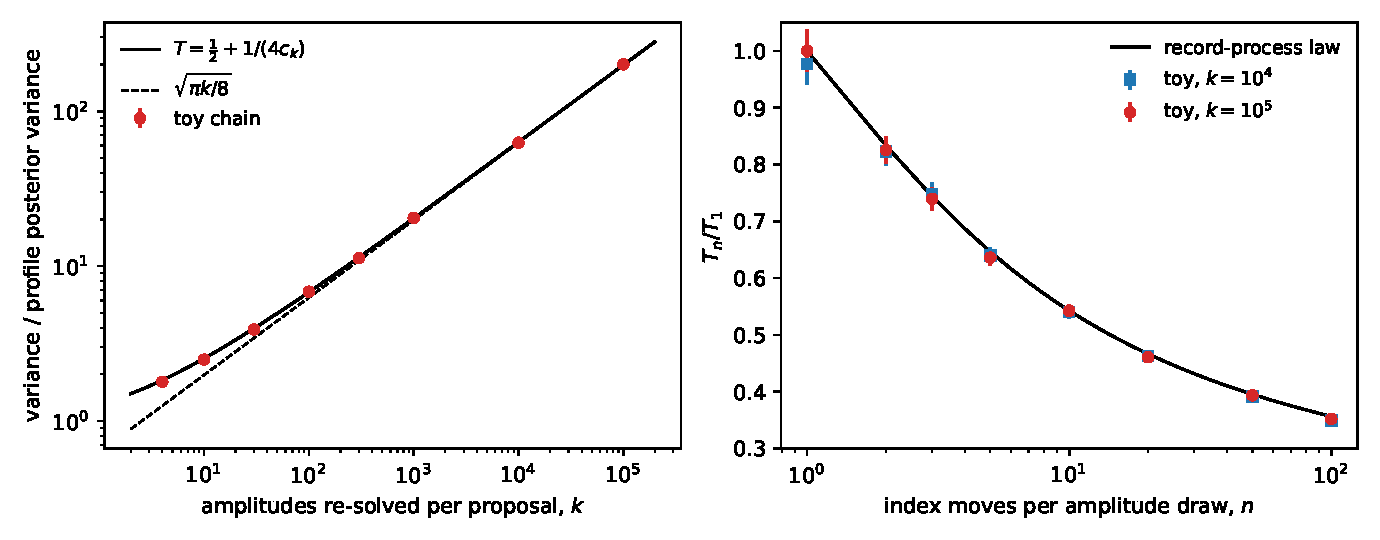
\includegraphics[width=0.98\textwidth]{figures/fig_temper.pdf}
\caption{The stationary law of the re-solve move inside a Gibbs sweep. Left: temperature of the
tempered profile posterior against the number of amplitudes re-solved per proposal, for one index
move per amplitude draw: Eq.~(\ref{eq:Tk}) (line), its leading term (dashed) and the toy chain
(points). Right: the ratio $T_n/T_1$ for $n$ index moves per amplitude draw: the record-process
law of Eq.~(\ref{eq:Rn}) (line) and the toy at $k = 10^4$ and $10^5$ (points).}
\label{fig:temper}
\end{figure}

\subsection{What this means for existing chains}

A chain run with this move reports index uncertainties that are too wide by $\sqrt{T}$, a factor of
order ten at map-level $k$, with a mean close to the profile posterior. It does not sample the
flat-prior joint posterior that the rest of the Gibbs sweep assumes. The statement applies to the
move as defined in steps 1 to 3 with exact conditional draws. Samplers that propose the index and
then solve for the conditional mean, or that evaluate a marginal likelihood in the acceptance, are
different algorithms. Commander3's index samplers are of the latter kinds (we read the code and did
not run it).
